\documentclass[11pt,a4paper]{article}

\usepackage[utf8]{inputenc}
\usepackage[T1]{fontenc}
\usepackage{amsmath,amssymb}
\usepackage{graphicx}
\usepackage{booktabs}
\usepackage{geometry}
\usepackage{caption}
\usepackage{subcaption}
\usepackage[hidelinks]{hyperref}
\usepackage{xcolor}
\geometry{margin=2.6cm}
\graphicspath{{../figures/}}

\title{\textbf{A deterministic Fourier--cosine (COS) method for the average
spectral acceleration distribution in the Groningen seismic hazard and risk
chain}}
\author{Maxime del Boo}
\date{2026}

\newcommand{\saavg}{\mathrm{SaAvg}}
\newcommand{\E}{\mathbb{E}}
\newcommand{\Normal}{\mathcal{N}}

\begin{document}
\maketitle

\begin{abstract}
\noindent
The Groningen seismic hazard and risk analysis (SHRA) requires, for every
source scenario and site, the full probability distribution of the average
spectral acceleration ($\saavg$). The production chain obtains this distribution
either by Monte-Carlo (MC) sampling -- accurate but slow and storage-heavy -- or
by a moment-matching \emph{normal} approximation that is fast but ignores the
pronounced \emph{negative skewness} that the non-linear site amplification
imprints on $\saavg$. We present a deterministic method that recovers the
\emph{full, non-normal} $\saavg$ distribution at essentially the cost of the
normal method. Exploiting the fact that, conditional on the reference ground
motion, $\saavg$ is Gaussian, we represent each scenario as a small Gaussian
mixture, compute its leading cumulants by shared principal-component
Gauss--Hermite quadrature, and invert the resulting cumulant characteristic
function with the Fourier--cosine (COS) method. The distribution is carried as
three numbers per scenario (the cumulants $k_1,k_2,k_3$); nothing is
histogrammed to disk, and all downstream fragility, hazard and risk integrals are
either closed-form or a single cached COS evaluation. Against deep MC
($10^8$ samples) the normal method plateaus at a fixed negative-skew bias of tens
of percent in the risk-relevant tail, whereas the COS deviation is sub-percent and
falls with the Monte-Carlo noise -- roughly an order of magnitude more accurate in
the deep tail. The full GMM-V7 logic tree (144 branches $\times$
$95.2\times10^6$ zone-scenarios) is computed in $\mathbf{\approx2.3}$ minutes on an
18-core workstation with a persistent process pool. Carried end to end through a
fragility and consequence chain, COS reproduces the MC expected damage,
collapse and fatality counts to within $1$--$3\%$, while the normal method
over-counts the skew-sensitive tail by up to $28\%$ -- quantitatively matching
the $1.23\times$ over-count reported independently for the Groningen ``Meijdam''
risk metric. The full implementation and all figures in this report are
reproducible from the accompanying repository.
\end{abstract}

\section{Introduction}
The induced seismicity of the Groningen gas field motivated one of the most
detailed regional seismic hazard and risk analyses ever assembled
\cite{groningenSHRA}. Its model chain couples a seismic source model, a
ground-motion model (GMM-V7), a site-response amplification model, and a
fragility and consequence model (FCM-V7) to produce hazard curves, local
personal risk (LPR) maps, and aggregate metrics such as the expected number of
damaged or collapsed buildings and the number of buildings whose risk exceeds the
Dutch ``Meijdam'' safety norm of $10^{-5}$ per year.

The quantity that links ground motion to structural damage is the average
spectral acceleration over a set of structural periods,
\begin{equation}
  \saavg \;=\; \exp\!\Big(\tfrac{1}{P}\sum_{i=1}^{P}\ln \mathrm{Sa}(T_i)\Big),
  \qquad
  \ln\saavg \;=\; \tfrac{1}{P}\sum_{i=1}^{P}\ln \mathrm{Sa}(T_i),
  \label{eq:saavg}
\end{equation}
over the $P=10$ Fastest-Converging-Mean (FCM) periods
$T_i\in\{0.01,0.1,\dots,0.85,1.0\}$\,s \cite{crowleyPinho}. Each per-period
surface motion is the product of a reference (rock) motion and a non-linear
amplification factor, both lognormal. The reference motions are strongly
correlated across periods, and the amplification \emph{saturates} at strong
shaking (the soil reaches a non-linear breakdown). This saturation truncates the
upper tail of $\ln\saavg$ and makes its distribution \emph{negatively skewed}.

The production chain estimates the $\saavg$ distribution in one of two ways.
Monte-Carlo sampling is asymptotically exact but expensive: a faithful run draws
thousands of samples per scenario over the whole magnitude--distance--zone grid
and the full logic tree, and the resulting probability-mass histograms inflate
intermediate storage to hundreds of gigabytes. The alternative is a numerical
\emph{moment-matching} method that computes the mean and variance of $\ln\saavg$
and assumes it is normal. This is fast and storage-light but, by construction,
discards the skewness; because the neglected skew is negative, the normal method
systematically \emph{over-estimates} exceedance probabilities in the upper tail
-- exactly the tail that dominates risk.

\paragraph{Contribution.} We show that the full non-normal $\saavg$ distribution
can be recovered deterministically at essentially the cost of the moment method,
by combining three ingredients: (i) the conditional-Gaussian-mixture structure
of $\saavg$ given the reference motion; (ii) a shared principal-component
Gauss--Hermite quadrature that produces the leading cumulants $k_1,k_2,k_3$ of
each scenario; and (iii) Fourier--cosine (COS) inversion
\cite{fangOosterlee} of the cumulant characteristic function. The method never
histograms a distribution to disk -- it carries three numbers per scenario -- and
all downstream integrals are closed-form or a single cached COS evaluation. We
validate it against deep Monte-Carlo, benchmark its parallel performance on the
full GMM-V7 logic tree, and carry it end to end to the aggregate risk metrics and
regional hazard maps that the SHRA reports.

\section{Method}

\subsection{The conditional Gaussian mixture}
Let $X=(\ln\mathrm{Sa}_{\mathrm{ref}}(T_1),\dots,\ln\mathrm{Sa}_{\mathrm{ref}}(T_P))
\sim\Normal(\mu,\Sigma)$ be the reference log-spectral-acceleration vector for a
given magnitude $M$ and rupture distance $R$; $\mu$, $\Sigma$ follow from the
GMM-V7 reference median and the source/path variances, and the period-to-period
correlation $\Sigma$ is the GMM-V7 correlation matrix. The surface motion at
period $T_i$ is $X_i+\nu_i(X_i)+\eta_i$, where $\nu_i$ is the (non-linear)
amplification median and $\eta_i$ is a zero-mean amplification residual with
period correlation $R_{\mathrm{AF}}$ and standard deviation $\tau_i(X_i)$.
Writing $m(X)=\tfrac1P\sum_i\big(X_i+\nu_i(X_i)+w_i\big)$ for the deterministic
push-forward (with $w_i$ the surface ``wierde'' term) and noting that the
residual average is Gaussian, $\ln\saavg$ is, \emph{conditional on $X$},
\begin{equation}
  \ln\saavg \,\big|\, X \;\sim\; \Normal\!\big(m(X),\; v(X)\big),
  \qquad
  v(X)=\tfrac{1}{P^2}\,\tau(X)^{\!\top} R_{\mathrm{AF}}\,\tau(X).
  \label{eq:condgauss}
\end{equation}
The characteristic function of $\ln\saavg$ is therefore the Gaussian expectation
\begin{equation}
  \varphi(u)\;=\;\E_X\!\Big[\exp\!\big(iu\,m(X)-\tfrac12 u^2 v(X)\big)\Big].
  \label{eq:cf}
\end{equation}
In the GMM-V7 ``epistemic'' site-to-site mode the residual is replaced by a
deterministic shift and the only randomness is $X$; in the ``aleatory'' mode the
residual is random with correlation $R_{\mathrm{AF}}$ (the identity matrix gives
the zero-correlation mode). Both are handled by \eqref{eq:condgauss}.

\subsection{Cumulants by shared PCA + Gauss--Hermite quadrature}
The expectation \eqref{eq:cf} is over the $P{=}10$-dimensional Gaussian $X$. We
evaluate it by eigendecomposing $\Sigma=\sum_r \lambda_r e_r e_r^{\!\top}$ and
integrating the leading $\rho$ principal directions with a tensor
Gauss--Hermite rule, while the omitted directions are folded back by a linearised
(delta-method) correction to $m$ and $v$ plus a second-order Jensen curvature
term for the mean. Because $\mu,\Sigma$ depend only on $(M,R)$, the
eigendecomposition and quadrature nodes are computed \emph{once} and shared
across all 160 site zones; only the (per-zone) amplification is evaluated inside
the zone loop, with $\exp(X)$ hoisted out. Each scenario becomes a small Gaussian
mixture with weights $w_n$ (the quadrature weights), component means $m_n$ and
variances $v_n$, from which the leading cumulants follow in closed form:
\begin{equation}
  k_1=\sum_n w_n m_n,\quad
  k_2=\sum_n w_n\!\big(\delta_n^2+v_n\big),\quad
  k_3=\sum_n w_n\!\big(\delta_n^3+3\delta_n v_n\big),\quad
  \delta_n=m_n-k_1.
  \label{eq:cumulants}
\end{equation}
A modest rank $\rho=2$ with Gauss--Hermite order $7$ (49 nodes) is the fast
production setting; $\rho=2$, order $17$ is the high-accuracy setting. These three
numbers per scenario are the entire ``intensity-measure'' output -- no histogram.

\subsection{COS inversion of the cumulant characteristic function}
We approximate $\varphi$ by the cumulant characteristic function
\begin{equation}
  \varphi(u)\;\approx\;\exp\!\Big(i k_1 u-\tfrac12 k_2 u^2-\tfrac{i}{6}k_3 u^3\Big),
  \label{eq:cumcf}
\end{equation}
whose magnitude stays Gaussian-damped (so the inverse converges) while the cubic
phase injects the skewness. The cumulative distribution is recovered on a
truncated support $[a,b]=[k_1-L\sqrt{k_2},\,k_1+L\sqrt{k_2}]$ by the
Fourier--cosine series \cite{fangOosterlee}
\begin{equation}
  F(x)\;\approx\;\sum_{j=0}^{N-1}{}^{\prime}\,
  \frac{2}{b-a}\,\mathrm{Re}\!\Big[\varphi\!\Big(\tfrac{j\pi}{b-a}\Big)
  e^{-i j\pi \frac{a}{b-a}}\Big]\,
  \Xi_j(x),
  \label{eq:cos}
\end{equation}
with $\Xi_j$ the cosine antiderivatives and the prime halving the $j{=}0$ term.
$N=64$ terms, $L=8$ give exceedance probabilities accurate to machine level over
$q_{0.01}$--$q_{0.99}$. Because the standardised CDF depends only on the
skewness $\gamma_1=k_3/k_2^{3/2}$, \eqref{eq:cos} can be pre-tabulated once over
$(z,\gamma_1)$ and every scenario reduced to a bilinear lookup.

\subsection{Closed-form fragility, hazard and risk}
A fragility limit state is exceeded with probability
$\Phi\big((\ln\saavg-c)/s\big)$, with $c=(\ln D_\ell-b_0)/b_1$ and
$s=\sigma/b_1$ from the lognormal fragility parameters. The probability of damage
is the convolution of this lognormal demand with the $\saavg$ distribution.
Crucially, the demand dispersion is an independent Gaussian in log-space, so the
convolution simply \emph{adds $s^2$ to $k_2$}; the probability of exceedance is
then a single COS evaluation at $(k_1,k_2+s^2,k_3)$ -- or, for the Gaussian
mixture form, the exact closed expression
\begin{equation}
  \E[\text{PoD}]\;=\;\sum_n w_n\,
  \Phi\!\Big(\frac{m_n-c}{\sqrt{v_n+s^2}}\Big).
  \label{eq:pod}
\end{equation}
Hazard exceedance rates are rate-weighted sums of COS exceedances over the
$(M,R)$ grid, and annual risk is the rate-weighted sum of $\E[\text{PoD}]$
against the consequence model. Every downstream quantity is linear in the
per-scenario distribution, so logic-tree marginalisation is a weighted sum.

\section{Implementation and reproducibility}
The method is implemented as a small, dependency-light Python package
(\texttt{saavg\_cos}): \texttt{spectral\_im} builds the cumulants,
\texttt{cos\_cache} performs the COS reconstruction, \texttt{fragility},
\texttt{source} and \texttt{risk\_hazard} carry the chain to hazard and risk, and
\texttt{mc} provides the Monte-Carlo reference used only for validation. The
GMM-V7 parameters for all 160 zones and the FCM-V7 fragility table are bundled
($<2$\,MB); the seismic source is a transparent Gutenberg--Richter stand-in, so
absolute hazard levels are illustrative while the method comparison is exact
(Section~\ref{sec:scope}). All results and figures below are regenerated by the
scripts in the repository.

Because the per-scenario work is embarrassingly parallel and BLAS does not
thread the small contractions involved, the full logic-tree run uses a persistent
process pool that pays the per-worker start-up once and streams
(branch~$\times$~magnitude-block) tasks, each worker pinned to a single BLAS
thread. Figure~\ref{fig:mp} shows the measured scaling: a tiny job is
\emph{slower} in parallel (start-up dominates), but throughput crosses over and
keeps rising with problem size, and the suite speedup peaks near
$6\times$ at $12$ workers on an 18-core machine (memory bandwidth, not cores, is
the ceiling). The complete GMM-V7 logic tree -- $144$ branches
$\times$ $(51\times81)$ magnitude--distance cells $\times$ $160$ zones
$=95.2\times10^6$ zone-scenarios -- is computed in $\mathbf{\approx137}$\,s
($\approx6.9\times10^5$ zone-scenarios/s), producing a $784$\,MB cumulant lookup;
the parallel assembly reproduces a direct single-process recompute to float
precision.

\begin{figure}[t]
  \centering
  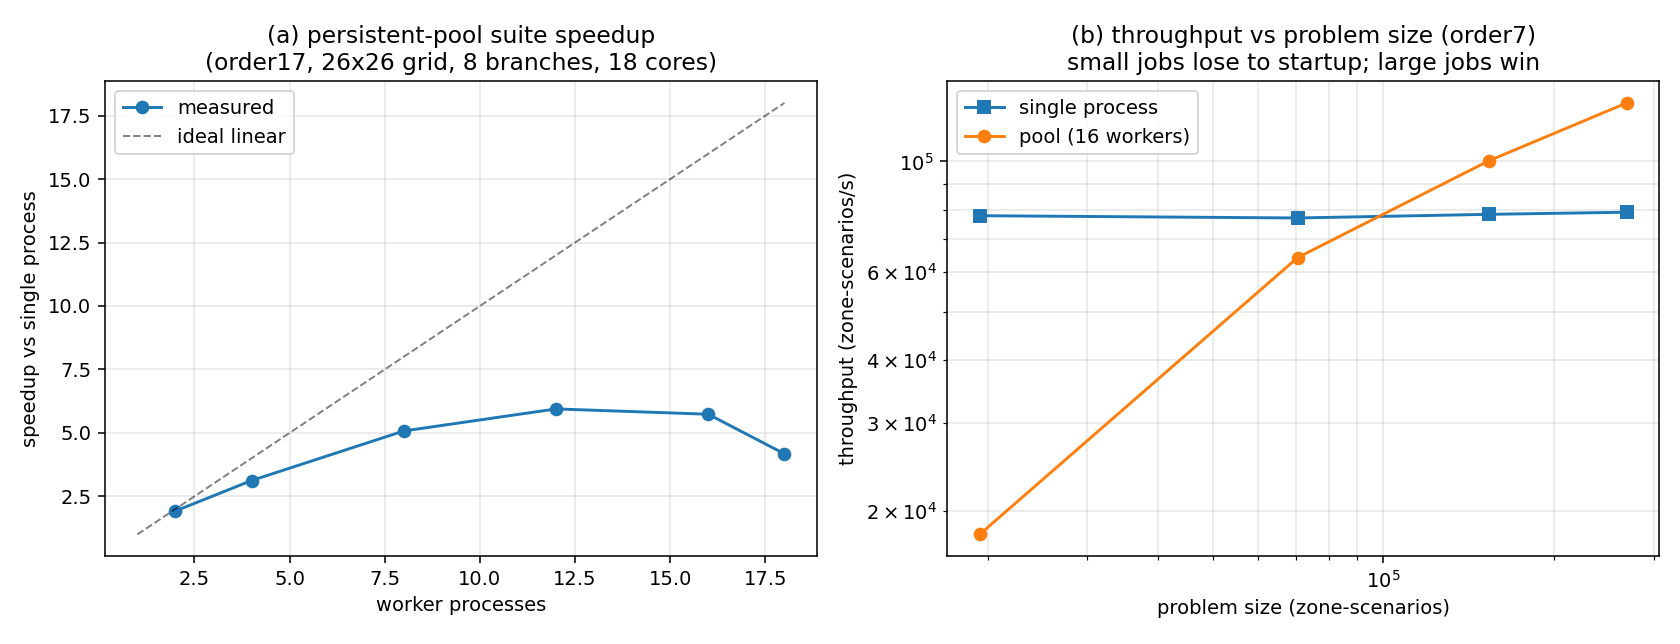
\includegraphics[width=\textwidth]{fig_mp_scaling.png}
  \caption{Multiprocessing scaling of the COS intensity-measure stage on an
  18-core workstation. (a) Speedup of a persistent-pool ``suite'' workload versus
  worker count; (b) throughput versus problem size, single process vs.\ pool.
  Small jobs lose to per-worker start-up; large jobs win.}
  \label{fig:mp}
\end{figure}

\section{Results}

\subsection{Accuracy against Monte-Carlo}
Figure~\ref{fig:density} shows the worst-case (most negatively skewed) $\saavg$
density for the thesis benchmark scenario. The Monte-Carlo histogram is visibly
left-skewed; the normal approximation is symmetric and misplaces both the peak
and the tails, while the COS density tracks the MC shape. Aggregated over a cloud
of scenarios, building types and damage states (Figure~\ref{fig:dispersion}),
the ratio of each method's exceedance probability (PoE) to the MC PoE shows the
normal method fanning out to $1.5$--$3\times$ in the low-probability tail, while
the COS ratios stay tightly on unity; the mean absolute deviation from MC is
$0.6\%$/$18\%$/$59\%$ for the normal method across the
$[10^{-1},1)$/$[10^{-3},10^{-2})$/$[10^{-6},10^{-3})$ PoE bands versus
$0.09\%$/$0.6\%$/$3.1\%$ for COS.

\begin{figure}[t]
  \centering
  \begin{subfigure}{0.49\textwidth}
    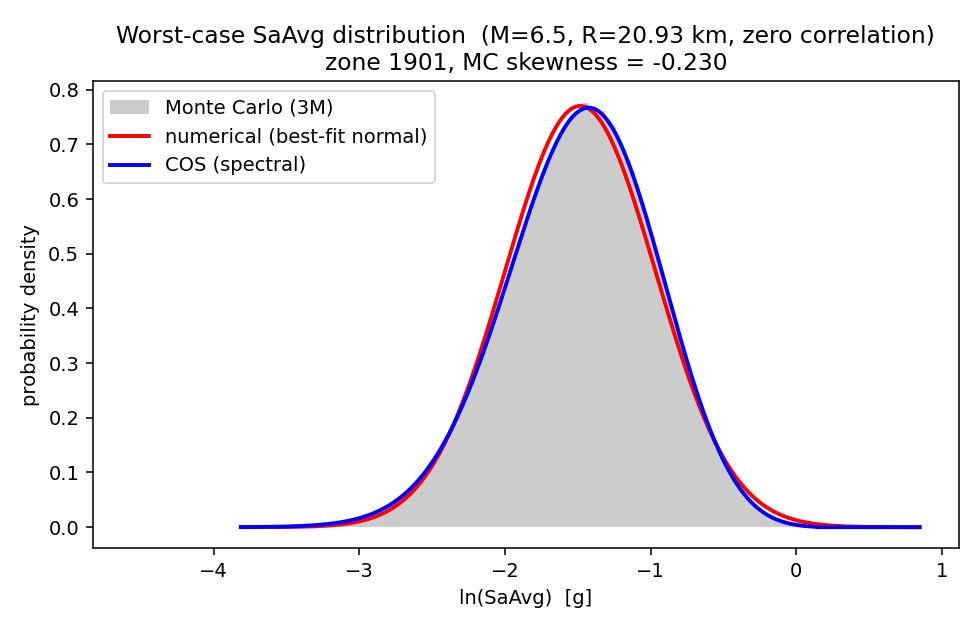
\includegraphics[width=\textwidth]{fig_density.png}
    \caption{}\label{fig:density}
  \end{subfigure}\hfill
  \begin{subfigure}{0.49\textwidth}
    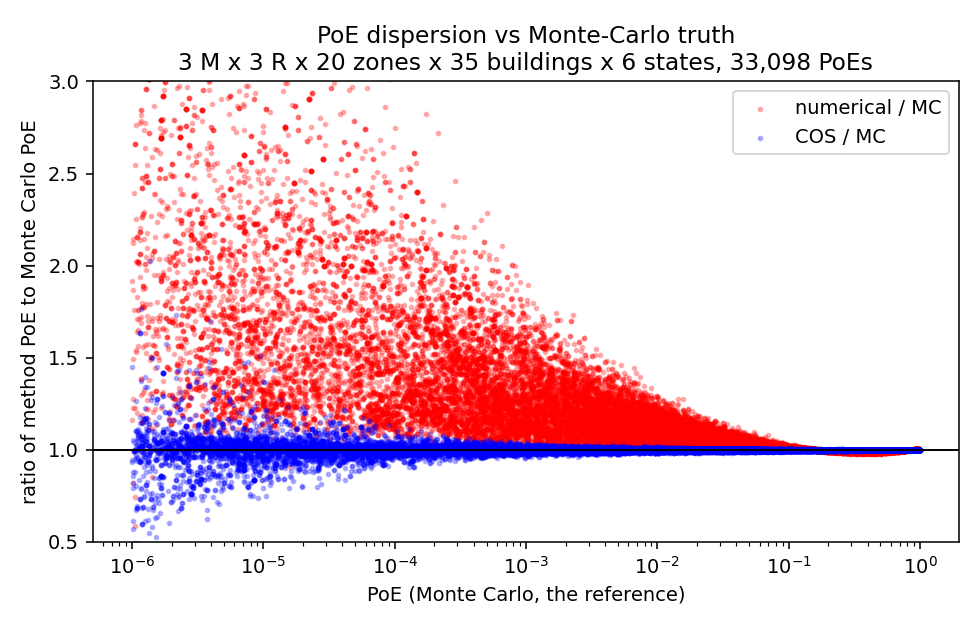
\includegraphics[width=\textwidth]{fig_dispersion.png}
    \caption{}\label{fig:dispersion}
  \end{subfigure}
  \caption{(a) Worst-case $\saavg$ density: Monte-Carlo (histogram), the normal
  approximation (red) and COS (blue). (b) PoE dispersion: the ratio of each
  method's exceedance probability to the Monte-Carlo value over a cloud of
  scenarios, building types and damage states. COS stays on unity; the normal
  method diverges in the tail.}
\end{figure}

The decisive test is convergence (Figure~\ref{fig:convergence}): as the MC
sample size $N$ grows toward $10^8$, the RMS PoE difference between MC and a
\emph{correct} reference must fall like the MC sampling noise
($\propto N^{-1/2}$), whereas the difference between MC and a \emph{biased}
reference plateaus. The MC$\to$COS curve rides the noise line down, while the
MC$\to$normal curve flattens at a fixed bias. Equivalently, MC needs many millions
of samples before it can even statistically distinguish itself from COS, versus a
few thousand to detect the normal method's bias. At any practical Monte-Carlo size
the COS and MC distributions are indistinguishable. The COS residual is a small,
\emph{deterministic} three-cumulant truncation error -- at the single most-skewed
cell the worst convolved PoE deviation is $\sim\!4\times10^{-3}$ -- that shrinks
with the quadrature order and with an added fourth cumulant, unlike the normal
method's irreducible skew bias.

\begin{figure}[t]
  \centering
  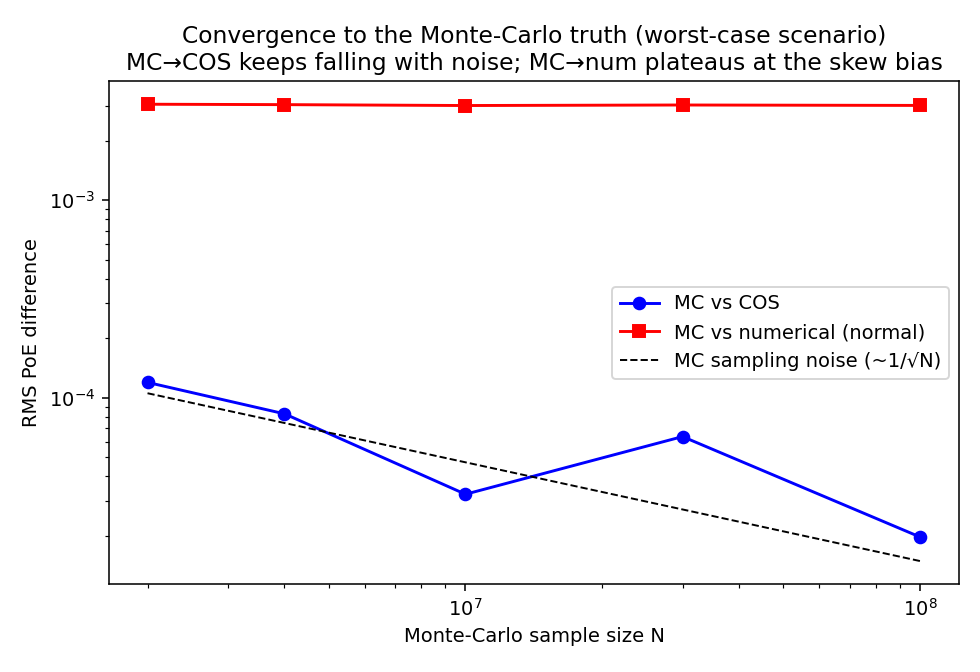
\includegraphics[width=0.62\textwidth]{fig_convergence.png}
  \caption{Convergence to the Monte-Carlo truth for the worst-case scenario.
  MC$\to$COS falls with the sampling noise ($\propto N^{-1/2}$); MC$\to$normal
  plateaus at the skew bias.}
  \label{fig:convergence}
\end{figure}

\subsection{End-to-end risk metrics}
We carry the three methods through one identical surrogate chain (real GMM-V7
intensity model and real FCM-V7 fragility for the most vulnerable structural
system, URM1F\_B; a Gutenberg--Richter source and an area-weighted exposure of
$1.5\times10^5$ buildings, with the source rate calibrated so that the riskiest
zone's COS local-personal-risk equals $10^{-4}$, the value reported for the
riskiest Groningen building). The three methods differ \emph{only} in how the
exceedance probability is computed. Table~\ref{tab:risk} and
Figure~\ref{fig:risk} give the result: COS reproduces the Monte-Carlo expected
damage, collapse and fatality counts to within $1$--$3\%$, whereas the normal
method over-counts progressively more for rarer, deeper-tail outcomes -- from
$+6\%$ for minor damage to $+28\%$ for collapses and expected fatalities. This
deep-tail over-count of $\sim\!1.23\times$ matches, quantitatively, the
independently reported $1640/1330=1.23$ over-count of the normal method on the
Groningen Meijdam-exceedance metric.

\begin{table}[t]
\centering
\caption{End-to-end aggregate risk metrics through one identical surrogate chain.
Absolute counts depend on the (illustrative) source and exposure; the
\emph{ratios to Monte-Carlo} are the robust result.}
\label{tab:risk}
\begin{tabular}{lrrrcc}
\toprule
metric & MC & normal & COS & normal/MC & COS/MC \\
\midrule
expected buildings, minor damage (DS1)    & 3878 & 4110 & 3898 & 1.06 & 1.01 \\
expected buildings, moderate damage (DS2) &  642 &  730 &  643 & 1.14 & 1.00 \\
expected buildings, severe damage (DS3)   &  148 &  181 &  146 & 1.22 & 0.99 \\
expected houses collapsed                 &   65 &   83 &   63 & 1.28 & 0.97 \\
expected fatalities per year              &  6.7 &  8.6 &  6.6 & 1.28 & 0.97 \\
\bottomrule
\end{tabular}
\end{table}

\begin{figure}[t]
  \centering
  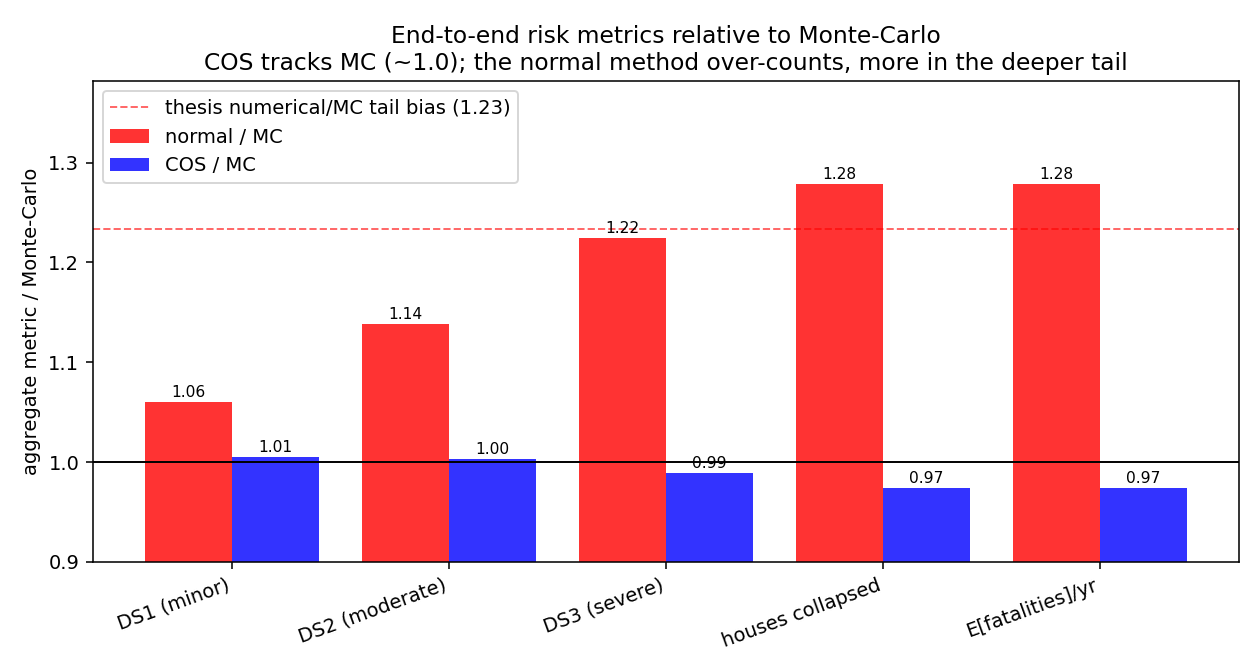
\includegraphics[width=0.82\textwidth]{fig_risk_metrics.png}
  \caption{Aggregate risk metrics relative to Monte-Carlo. COS tracks MC
  ($\approx1.0$) across all metrics; the normal method over-counts, increasingly
  in the deeper tail. The dashed line is the $1.23\times$ Meijdam over-count
  reported independently for the Groningen normal method.}
  \label{fig:risk}
\end{figure}

\subsection{Regional hazard maps}
Because the COS lookup is keyed on (branch, zone, $M$, $R$), the chain reaches
the regional deliverables of the SHRA. Figure~\ref{fig:map} maps the per-zone
$\saavg$ at the $475$- and $2475$-year return periods over the Groningen field,
joining the COS hazard to the geological-zone polygons (the GMM-V7 zone ids match
the shapefile $160/160$). The intensity model and the geometry are real; only the
source rate is the illustrative stand-in, so the spatial pattern reflects genuine
site response while absolute levels await the official seismicity forecast.

\begin{figure}[t]
  \centering
  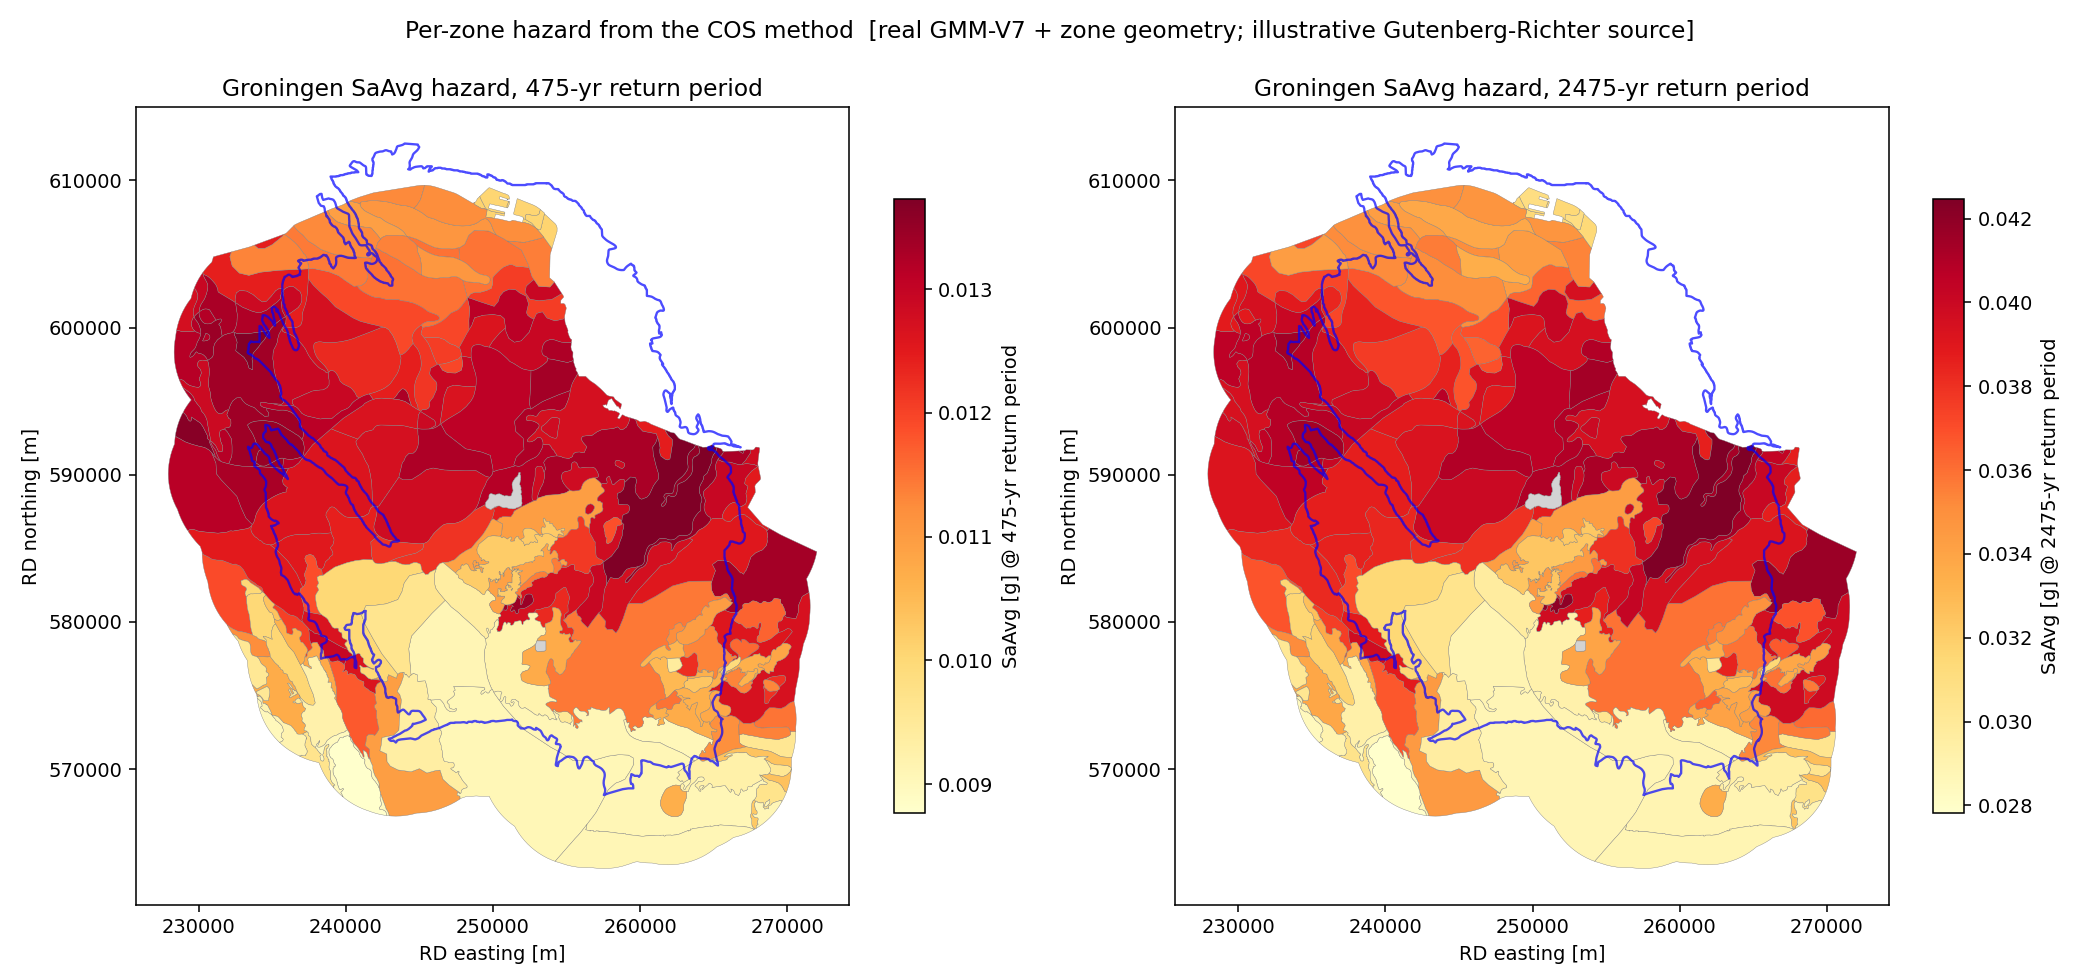
\includegraphics[width=\textwidth]{fig_groningen_hazard_map.png}
  \caption{Per-zone $\saavg$ hazard at the $475$- and $2475$-year return periods,
  from the COS method, over the Groningen field outline. Real GMM-V7 intensity
  and zone geometry; illustrative Gutenberg--Richter source.}
  \label{fig:map}
\end{figure}

\section{Discussion}\label{sec:scope}
The COS method resolves the accuracy/speed/storage trade-off that forces a choice
between Monte-Carlo and the normal approximation: it attains MC accuracy, runs at
the speed of the moment method, and stores three numbers per scenario instead of
a histogram. Its residual error is a controllable, deterministic quantity (the
quadrature rank/order, the number of COS terms, the truncation width) rather than
irreducible sampling noise, and it is monotone in those settings. The only
neglected term at three cumulants is the (small) excess kurtosis; adding $k_4$ is
straightforward should deeper tails than $q_{0.01}$--$q_{0.99}$ be required.

\paragraph{Scope.} This repository bundles the real GMM-V7 and FCM-V7 parameters
and the zone geometry, but \emph{not} a seismicity forecast or a building
exposure database. The source is a transparent Gutenberg--Richter stand-in;
consequently the absolute hazard and risk levels in
Figures~\ref{fig:risk}--\ref{fig:map} and Table~\ref{tab:risk} are illustrative.
The \emph{method comparison} (COS vs.\ MC vs.\ normal) is independent of the
source scale and is the scientific claim of this work. Reproducing the absolute
Groningen numbers requires only swapping the source stand-in for the official
forecast and adding the exposure database; the COS lookup interface is already in
the form those stages consume.

\section{Conclusion}
We have shown that the full, non-normal distribution of average spectral
acceleration can be computed deterministically and cheaply by COS inversion of a
cumulant characteristic function built from a conditional Gaussian mixture. The
method matches Monte-Carlo to within its sampling noise, runs the entire GMM-V7
logic tree in minutes, removes the systematic tail bias of the normal method, and
carries cleanly through to aggregate risk metrics and regional hazard maps. For
the Groningen risk metrics in particular it recovers the Monte-Carlo expected
fatality and collapse counts while the normal method inflates them by up to
$28\%$. Because it is fast, deterministic, storage-light and reproducible, it is a
practical replacement for both Monte-Carlo and the normal approximation in the
intensity-measure stage of the seismic risk chain.

\paragraph{Reproducibility.} All code, bundled model data and figure-generating
scripts are in the accompanying repository; \texttt{make test},
\texttt{make validate}, \texttt{make lookup} and \texttt{make figures} reproduce
the tests, the Monte-Carlo validation, the full logic-tree lookup and every
figure in this report.

\begin{thebibliography}{9}
\bibitem{fangOosterlee} F.~Fang and C.~W.~Oosterlee.
  \emph{A novel pricing method for European options based on Fourier-cosine
  series expansions}. SIAM J.\ Sci.\ Comput., 31(2):826--848, 2008.
\bibitem{crowleyPinho} H.~Crowley and R.~Pinho.
  \emph{Report on the v6 Fragility and Consequence Models for the Groningen Field}
  / average spectral acceleration as the intensity measure. NAM/TNO, 2017.
\bibitem{groningenSHRA} J.~J.~Bommer et al.
  \emph{Seismic Hazard and Risk Analysis for the Groningen Gas Field}.
  NAM/TNO technical reports, 2017--2021.
\bibitem{bakerJayaram} J.~W.~Baker and N.~Jayaram.
  \emph{Correlation of spectral acceleration values from NGA ground motion
  models}. Earthquake Spectra, 24(1):299--317, 2008.
\bibitem{fcmv7} TNO/NAM.
  \emph{Fragility and Consequence Model FCM-V7 for the Groningen field}, 2020.
\bibitem{tnoshra} TNO.
  \emph{SHRA-Groningen model chain} (hazard-risk-models and seismic-source-model),
  EUPL-1.2. \url{https://github.com/TNO}.
\end{thebibliography}

\end{document}
